\documentclass[11pt]{article}

\usepackage{geometry}
\geometry{margin = 1in,top =0.12\paperheight, headheight=\paperheight}
\usepackage[export]{adjustbox}
\usepackage{array}
\usepackage{amsmath}
\usepackage{amsfonts}
\usepackage{fancyhdr}
\usepackage{lastpage}
\usepackage{xcolor}
\pagestyle{fancy}
\fancyhf{}
\rhead{Written Assignment, Page \thepage}
\lhead{MATH211}
\chead{
\includegraphics[width = 0.15\textwidth]{MCLogo-Bck.png}}


%\renewcommand{\footrulewidth}{0.4pt}

\usepackage{enumitem}
\usepackage{pifont}
\usepackage{graphicx}
\graphicspath{{../img/}}

\newtheorem{theorem}{Theorem}
\newtheorem{exercise}{Exercise}


\newcommand{\R}{\mathbb R}
\newcommand{\e}{{\rm e}}
\newcommand{\inpr}[1]{\left\langle#1\right\rangle}
\newcommand{\norm}[1]{\lVert #1 \rVert}
\newcommand{\abs}[1]{\lvert #1 \rvert}
\newcommand{\vv}{\mathbf v}
\newcommand{\uv}{\mathbf u}

\DeclareMathOperator{\xd}{d\!}
\DeclareMathOperator{\proj}{proj}

\title{}
\date{}

\begin{document}
\noindent {\bf Problem.}
Review the lecture notes and read the paragraph above Figure 11.17 in the textbook, then flesh out the details of the derivation of the formula for the distance between two points in space:
\[
d = \sqrt{(x_2-x_1)^2 + (y_2-y_1)^2 + (z_2-z_1)^2}.
\] 
\begin{figure}[h]
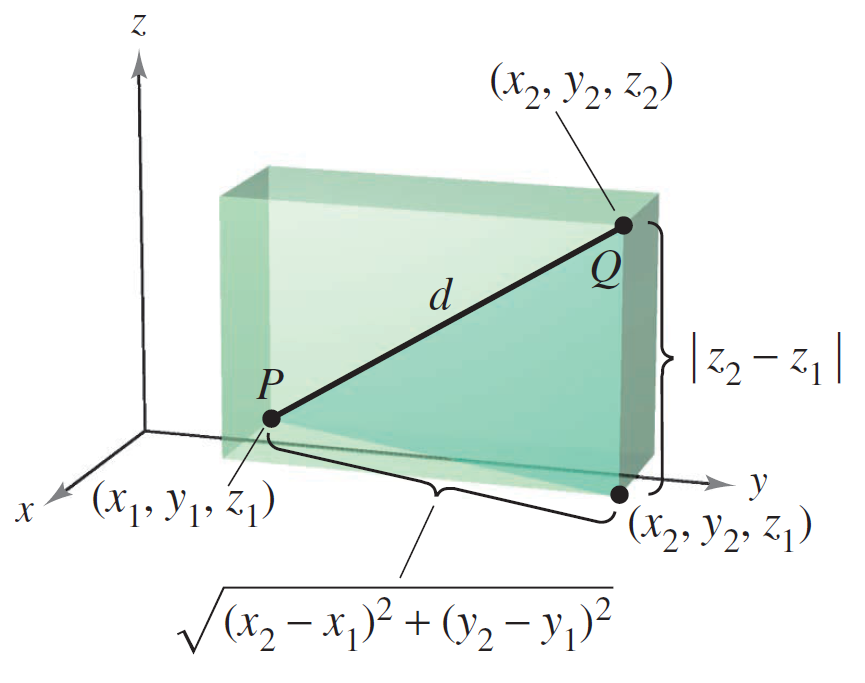
\includegraphics[width = 0.4\textwidth,right]{distformula.png}
\end{figure}

\end{document}